\documentclass[PICOAPC.tex]{subfiles}
\newcommand\pdeg{.\!\!\degree}
\newcommand\parcm{.\!\!'}

\section{Technical Overview}
\label{sec:techoverview}

PICO meets all of its science-driven instrument requirements with a single instrument: an imaging polarimeter with 21 logarithmically spaced frequency bands centered between 21 and 799\,GHz (Table~\ref{tab:bands}). The instrument has a two-reflector Dragone-style telescope; see Figure.~\ref{fig:InstrumentCAD}. The focal plane is populated by \ac{TES} bolometers and read out using a time-domain multiplexing scheme. The instrument has both passive and active cooling stages. PICO operates from the Earth-Sun L2 and employs a single science observing mode, providing highly redundant coverage of the full sky. A full description of the reference design is given by \citet{pico_report}.

\begin{figure}[h] 
\hspace{-0.1in}
\parbox{4.8in}{\centerline{
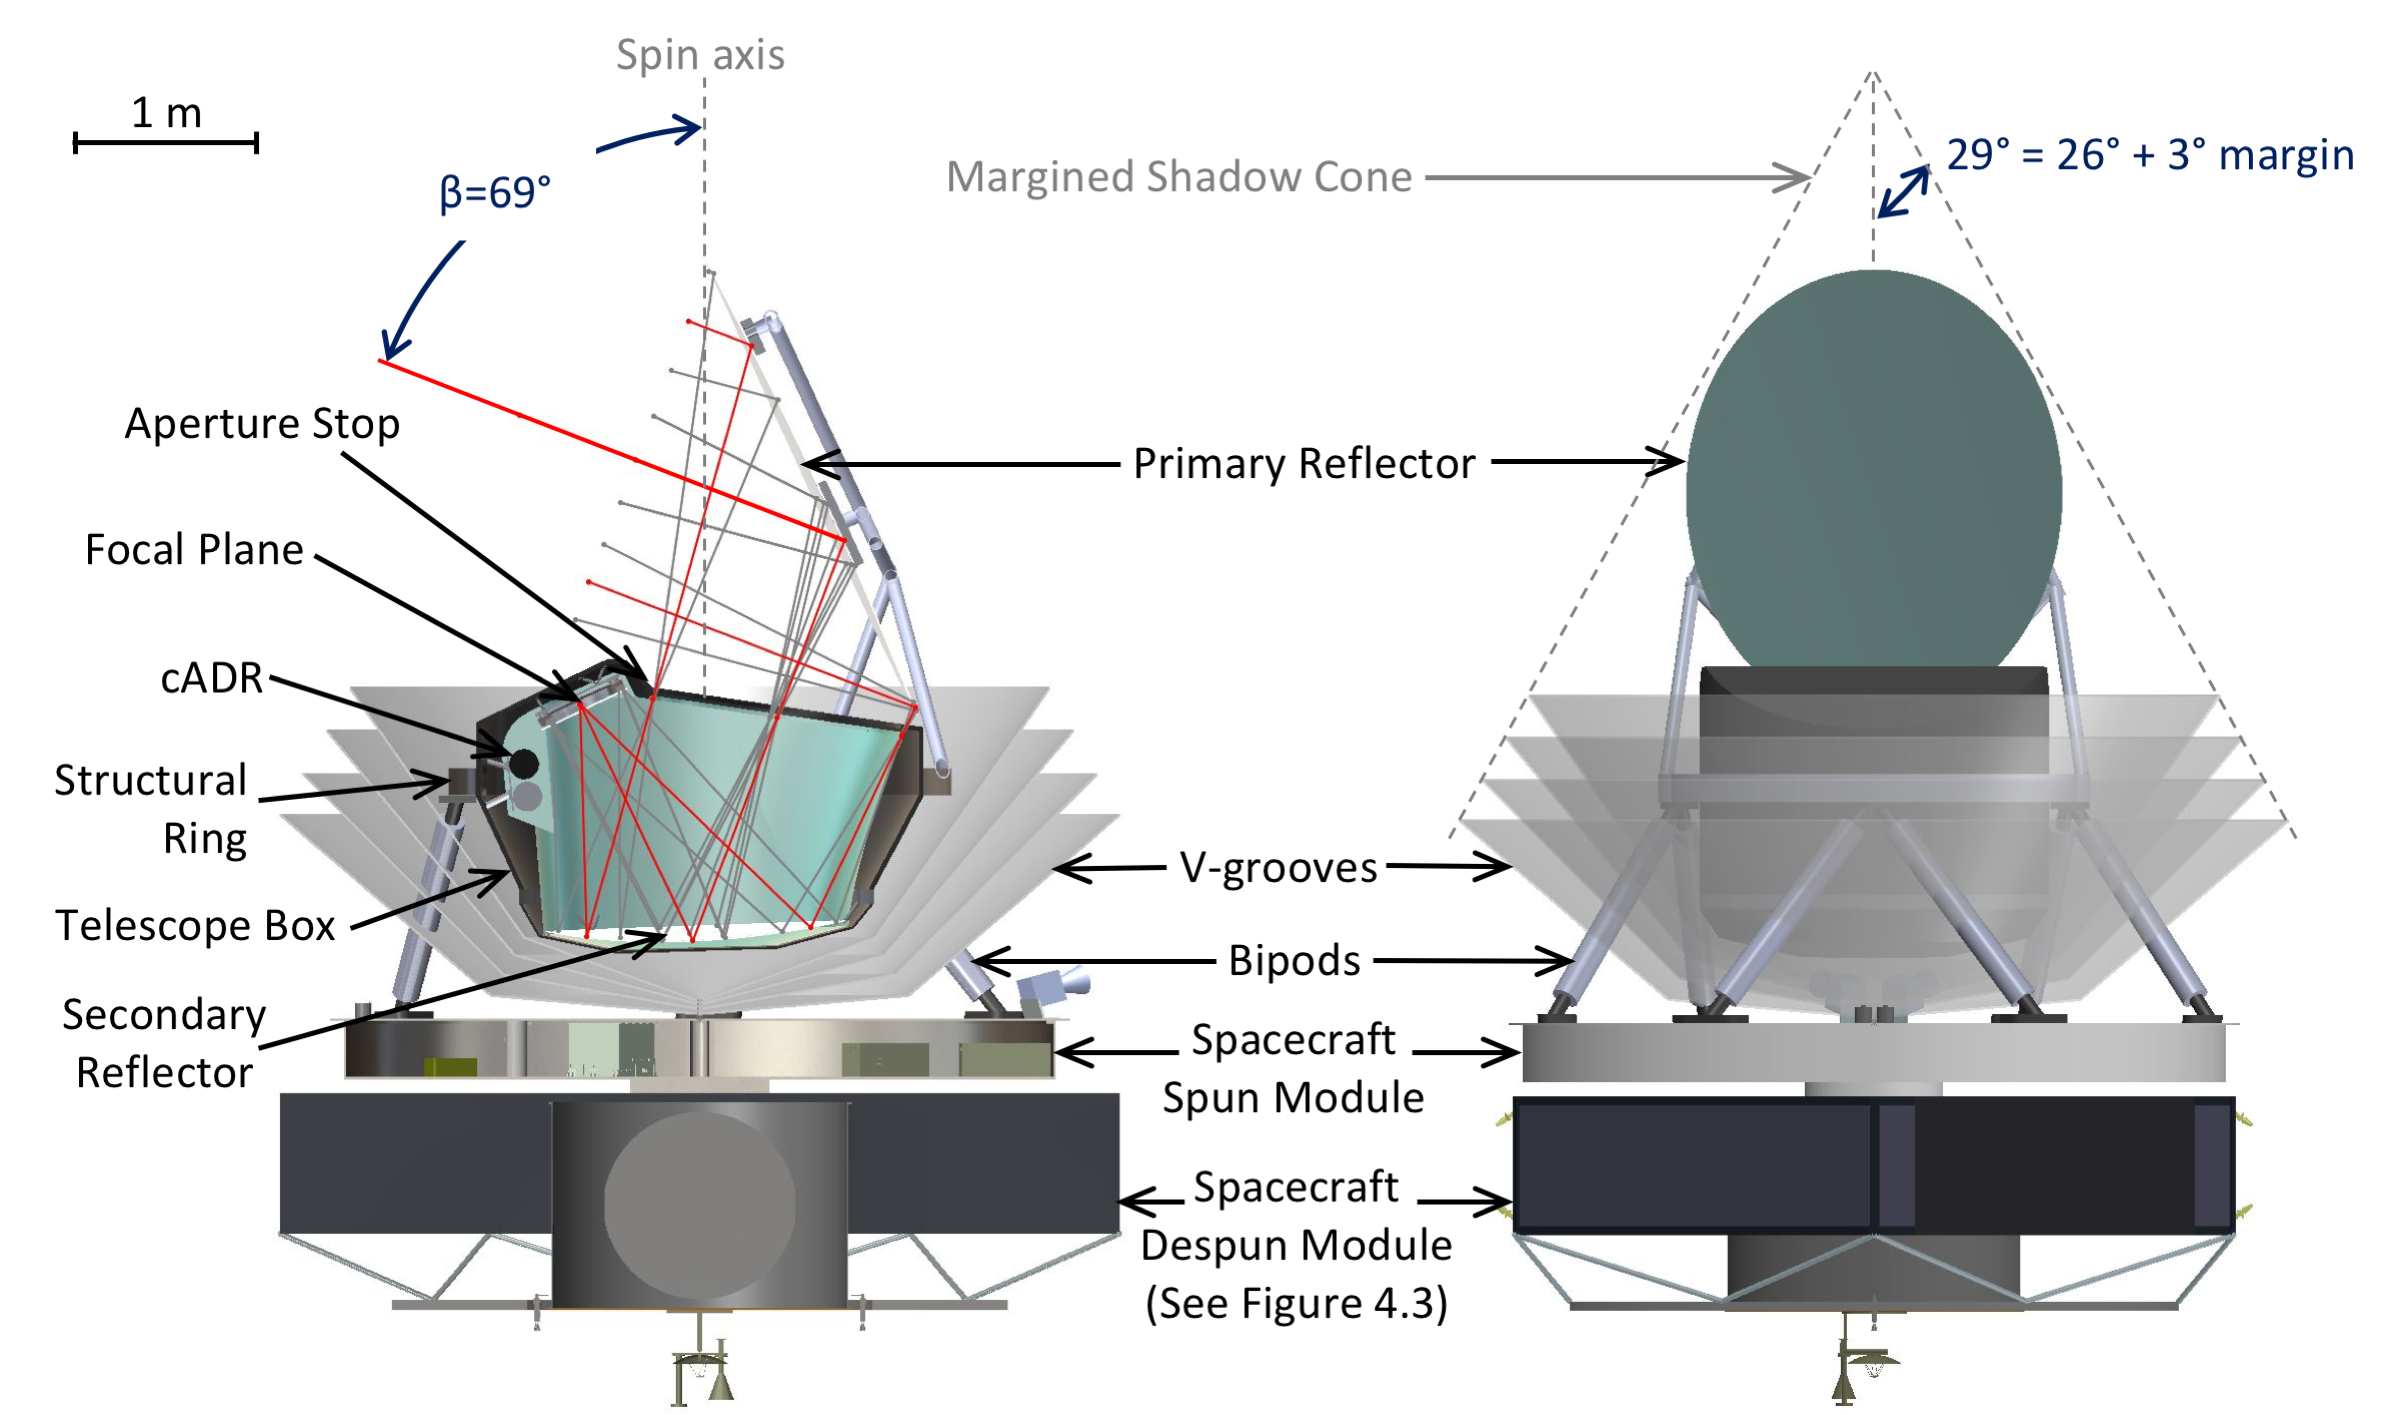
\includegraphics[width=4.8in]{figures/InstrumentCAD.png} }}
\hspace{0.0in}
\parbox{1.6in}{
\caption{\captiontext
PICO overall configuration in side view and cross section (left), and front view with V-Groove assembly shown semi-transparent (right).  The mission consists of a single science instrument mounted on a structural ring. The ring is supported by bipods on a stage spinning at 1~RPM relative to a despun module. Only power and digital information pass between the spun and despun stages. 
\label{fig:InstrumentCAD}} }
%\end{center}
\vspace{-0.15in}
\end{figure}

%% begin wcj comment - move to scan section

%During the survey, the instrument is spun at 1~rpm and the spin axis is made to precess about the anti-Sun direction (\S\,\ref{sec:survey_design}). Spacecraft control is simplified by mounting the instrument on a spinning spacecraft module, while a larger non-spinning module houses most spacecraft subsystems (\S\,\ref{sec:spacecraft}). Instrument elements that act as heat sources are accommodated on the spinning module of the spacecraft. Only power and digital data lines cross between the spinning and non-spinning modules.

%% end wcj comment

\subsection{Telescope, Detectors, and Readout}
\label{sec:telescope} 

The PICO telescope gives a large diffraction-limited field of view, sufficient to support approximately $10^4$ detectors; arcminute resolution at 800\,GHz; low instrumental and cross-polarization; and low sidelobe response. All requirements are met with PICO's 1.4\,m aperture modified open-Dragone design. There are no moving parts in the PICO optical system. There are no lenses, eliminating absorption and reflection losses and obviating the need for anti-reflection coatings. The primary mirror is passively cooled to $\sim$20~K. An aperture stop and a secondary mirror are actively cooled to 4.5~K. 

The sensitivity of PICO's detectors is limited by irreducible backgrounds: the CMB at frequencies below 400~GHz, and emission from the cold primary mirror at higher frequencies. Therefore, the required sensitivity determines the detector count in each band. The PICO focal plane has 12,996 detectors, 175~times the number flown aboard \planck , thereby providing the required increase in raw sensitivity.  To achieve similar raw sensitivity to PICO, a ground-based instrument would require $\sim$50 times the number of detectors, and therefore a massive array of cryogenic receivers.  

The PICO baseline focal plane employs three-color sinuous antenna/lenslet pixels~\citep{Suzuki2014} for the 21--462\,GHz bands. Niobium microstrips mediate the signals between the antenna and detectors, and partition the wide continuous bandwidth into three narrow channels using integrated, on-wafer, micro-machined filter circuits~\citep{OBrient2013}. Six transition edge sensor bolometers per pixel detect the radiation in two orthogonal polarization states. 

PICO's highest three frequency channels are beyond the niobium superconducting band-gap, rendering on-wafer, microstrip filters a poor solution for defining the optical passband. For these bands we use feedhorns to couple the radiation to two single-color polarization-sensitive TES bolometers. The waveguide cut-off defines the lower edge of the band, and quasi-optical metal-mesh filters define the upper edge. Numerous experiments have successfully used similar approaches~\citep{Shirokoff2011,Bleem2012,Turner2001}. 

Polarimetry is achieved by measuring the signals from pairs of two co-pointed bolometers within a pixel that are sensitive to two orthogonal linear polarization states. Half the pixels in the focal plane are sensitive to the $Q$ and half to the $U$ Stokes parameters of the incident radiation, providing sensitivity to the Stokes $I$, $Q$, and $U$ parameters. Two layouts for the distribution of the $Q$ and $U$ pixels on the focal plane have been investigated~\citep{picoweb_QU}; both satisfy mission requirements. 

The current baseline for PICO is to use a time-domain multiplexer (TDM), because to date this scheme uses the least power consumption and dissipation at ambient temperatures. The thermal loading on the cold stages from the wire harnesses is subdominant to conductive loading through the mechanical support structures. In the PICO TDM implementation a row of 102 detectors are readout simultaneously, and 128 such rows are readout sequentially. SQUIDs will be used as current amplifiers. Suborbital experiments have developed techniques to shield the SQUIDs from Earth's magnetic field~\citep{Hui2018}.  Total suppression factors better than $10^7$ have been demonstrated~\citep{Runyan2010}. PICO will use these demonstrated techniques to shield SQUID readout chips from the ambient magnetic environment, which is 20,000 times smaller than near Earth. 

\subsection{Thermal}
\label{sec:thermal} 

The PICO thermal system does not require cryogenic consumables, permitting consideration of significant mission extension beyond the prime mission. The system, consisting of V-groove radiators for passive cooling, mechanical coolers to achieve 4.5~K, and a continuous adiabatic demagnetization refrigerator (cADR), meets all thermal requirements with robust margins~\citep{pico_report} .

A multi-stage continuous adiabatic demagnetization refrigerator (cADR) maintains the PICO focal plane at 0.1\,K and the surrounding enclosure, filter, and readout components at 1\,K. Heat loads in the range of 30~$\mu$W at 0.1\,K and 1\,mW at 1\,K (time-average) are within the capabilities of current cADRs developed by GSFC~\citep{Shirron2012,Shirron2016} and flown on suborbital balloon flights. The PICO sub-kelvin heat loads are estimated at less than half of this capability.

A cryocooler system similar to that used on JWST to cool the MIRI detectors~\citep{Durand2008,Rabb2013} backs the cADR and cools the aperture stop and secondary reflector to 4.5\,K. Both Northrop Grumman Aerospace Systems (NGAS, which provided the MIRI coolers) and Ball Aerospace have developed such coolers under the NASA-sponsored Advanced Cryocooler Technology Development Program~\citep{Glaister2006}. The NGAS project has completed PDR-level development, and is expected to reach CDR well before PICO begins Phase-A. The projected performance of this cooler will give more than 100\,\% heat lift margin relative to PICO's requirements~\citep{pico_report}.


\subsection{Instrument Integration and Test}
\label{sec:iandt} % 3.5

The PICO instrument integration and testing plan benefits from heritage and experience with the \planck\ HFI instrument~\citep{Pajot2010}.
Detector wafers are screened prior to selection of flight wafers and focal-plane integration. The cADR and 4\,K cryocooler vendors will qualify those subsystems prior to delivery. The relative alignment of the two reflectors is determined under in-flight thermal conditions using a thermal vacuum (TVAC) chamber and photogrammetry. The flight focal-plane assembly and flight cADR are integrated and tested in a dedicated sub-kelvin cryogenic testbed. The noise, responsivity, and focal-plane temperature stability are characterized using a representative optical load for each frequency band (temperature-controlled blackbody).  The same testbed is used to perform the  polarimetric and spectroscopic calibration.

The focal plane is integrated with the reflectors and structures, and alignment verified with photogrammetry at cold temperatures in a TVAC chamber.  The completely integrated observatory (instrument and spacecraft bus) is tested in TVAC to measure parasitic optical loading from the instrument, noise, microphonics, and RFI. The observatory is 4.5\,m in diameter and 6.1\,m tall. There are no deployables.

\subsection{Design Reference Mission}
\label{sec:design_reference} 

The PICO concept of operations is similar to that of the successful \wmap~\citep{Bennett2003} and \planck~\citep{Tauber2010} missions. After launch, PICO cruises to a quasi-halo orbit around the Earth--Sun L2 Lagrange point. A two-week decontamination period is followed by instrument cooldown, lasting about two months. After in-orbit checkout is complete, PICO begins its science survey. During the survey the instrument spins around the spacecraft's symmetry axis at 1~RPM. The symmetry axis precesses around the anti-sun direction with a period of 10~hours; See Figure~\ref{fig:MissionDesignFigure}. This survey ensures that each sky pixel is revisited along many orientations, which is optimal for polarimetric measurements. Nearly 50\% of the sky are surveyed every two weeks. The entire sky is covered in 6 months. Over the 5 year duration, PICO executes 10 independent full sky surveys, giving high redundancy for identifying systematic uncertainties. 

\begin{figure}[!b]
  \begin{minipage}[b]{0.29\textwidth}
    \begin{center}
    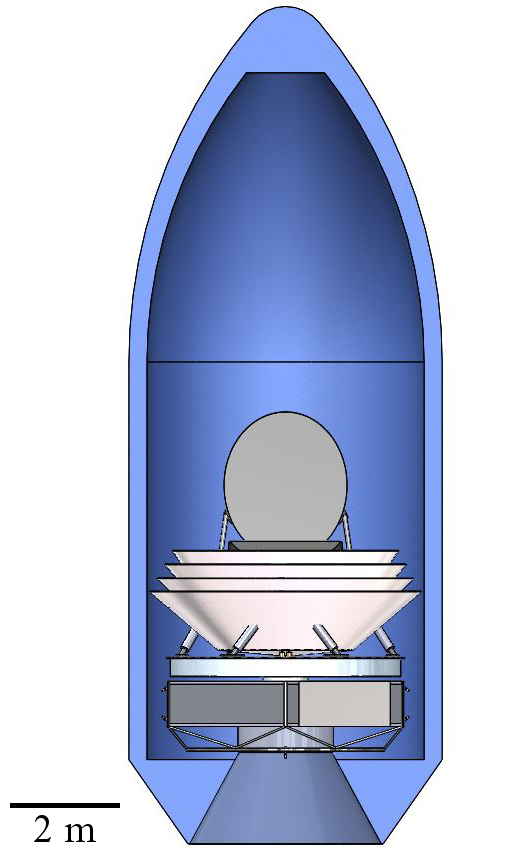
\includegraphics[width=1.5in]{figures/InFairing.JPG}
\caption{\captiontext PICO is compatible with the Falcon~9.\label{fig:InFairing}}
    \end{center}
  \end{minipage}
\hfill
\begin{minipage}[b]{0.67\textwidth}
    \begin{center}
    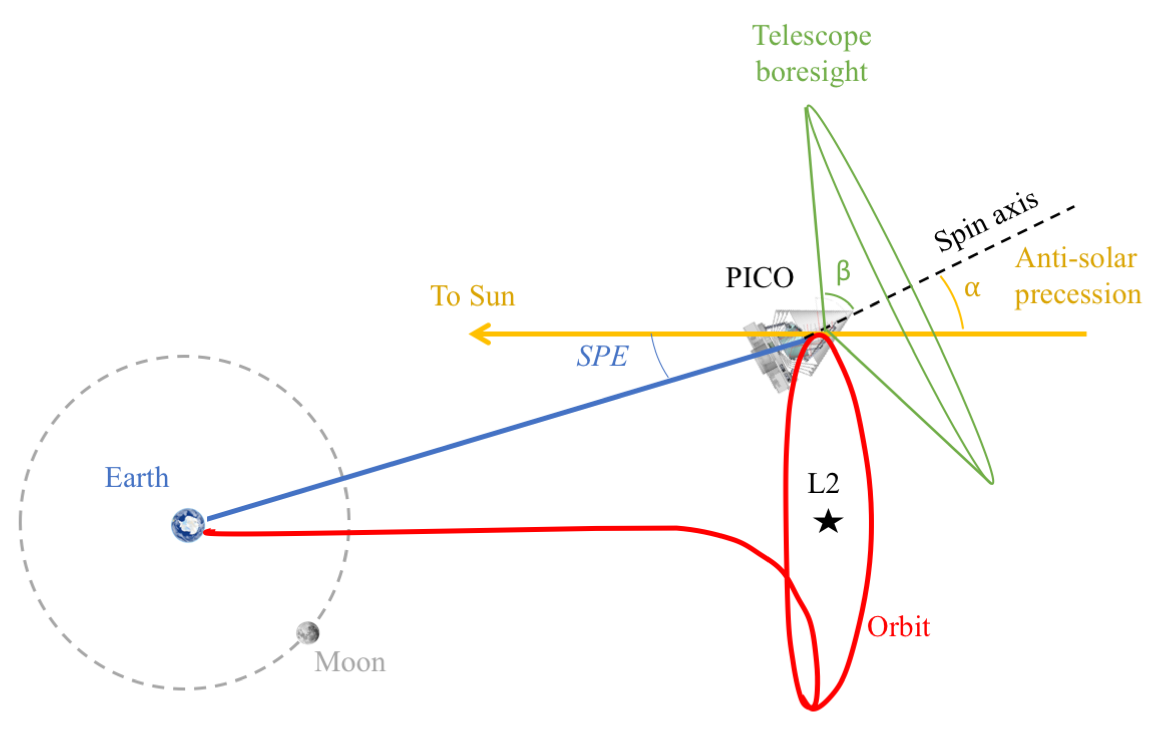
\includegraphics[width=4in]{figures/MissionDesignFigure.png}
\caption{\captiontext
  PICO surveys by continuously spinning the instrument about a
  precessing axis.\label{fig:MissionDesignFigure}}
   \end{center}
  \end{minipage}
\end{figure}

Instrument data are compressed and stored on-board, then returned to Earth in daily 4-hr Ka-band science downlink passes (concurrent with science observations). High data-rate downlink to the Deep Space Network (DSN) is available from L2 using near-Earth Ka bands. We assumed a launch with the Falcon~9. Its capability for ocean recovery exceeds PICO's 2147\,kg total launch mass (including contingency) by a $50\,\%$ margin.

The PICO spacecraft bus is Class~B and designed for a minimum lifetime of 5\,years in the L2 environment. Mission-critical elements are redundant. The aft end of the spacecraft (the ``de-spun module'') is comprised of six equipment bays that house standard components.  The instrument and V-grooves are mounted on bipods from the spacecraft's ``spun module,'' which contains the 4\,K cooler compressor and drive electronics, the sub-K cooler drive electronics, and the detector warm readout electronics. A motor drives the spun module at 1\,rpm. Only power and data (digital) lines pass between the spun and de-spun modules. Reaction wheels on the despun module cancel the angular momentum of the spun module and provide three-axis control.



%%% WCJ note: I don't see a need for this as a standalone section in the APC
%%%
%\bigskip
%\newpage
\subsection{Technology Drivers}
%\section{Technology Drivers}
%\label{sec:technology_maturation} %5
%
%\begin{wrapfigure}[10]{r}{3.80in}  % r is right aligned, l is left. Capital letters allow figure to float on page.
%\vspace{-15pt} % move figure up to align with section headings.
%\parbox{2.35in}{
%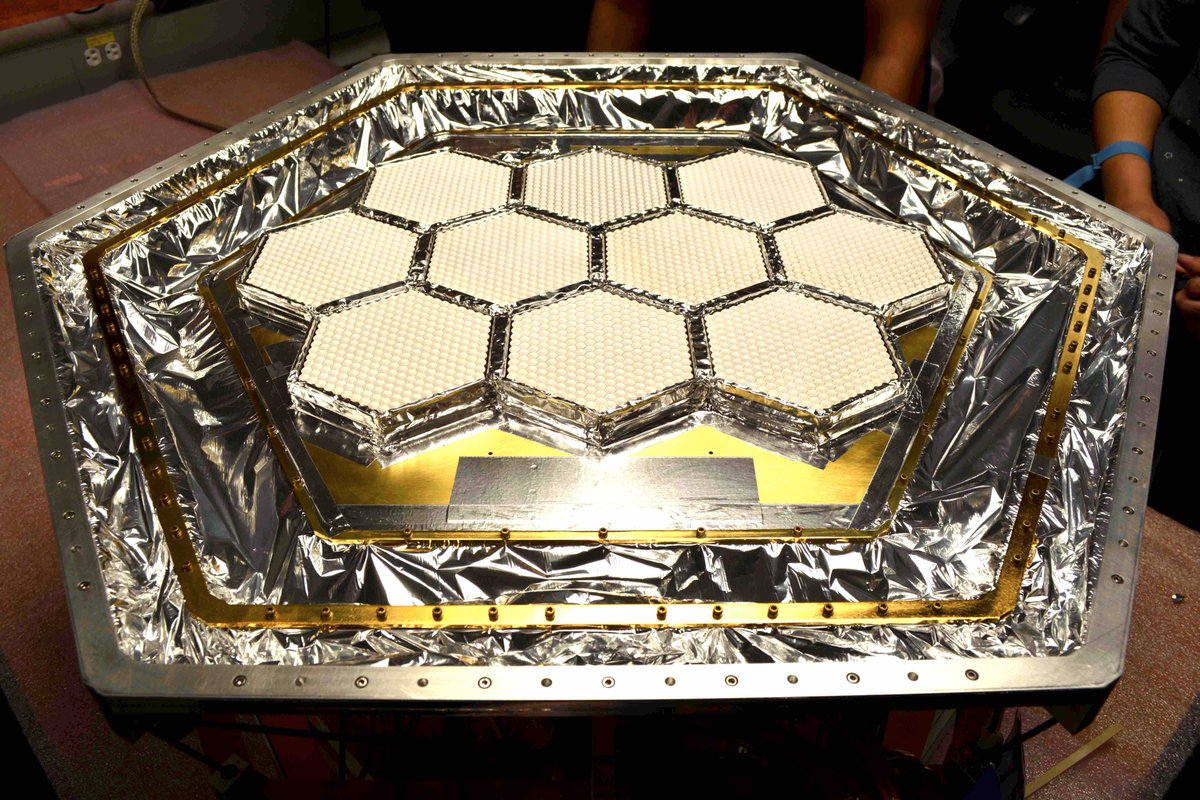
\includegraphics[width=2.35in]{figures/SPT3G.jpg} }  %% image was 3 in wide in past version.
%\parbox{1.40in}{
%\caption{\captiontext SPT-3G operates a focal plane with sinuous antenna-coupled, three-band pixels with 16,000 bolometers~\citep{Dutcher2018}. Each pixel couples radiation to bands at 95, 150, and 220~GHz.\label{fig:spt_fp} }
%}
%\end{wrapfigure}

PICO builds off of the heritage of \planck-HFI and \textit{Herschel}.  Since the time of \planck\ and \textit{Herschel}, suborbital experiments have used monolithically fabricated TES bolometers and multiplexing schemes to field instruments with thousands of \ac{TES} bolometers per camera (Fig.~\ref{fig:spt_fp}). %By the time PICO enters Phase~A, S3 experiments plan to be operating nearly 100,000 \ac{TES} bolometers in several independent cameras~\citep{Simons2018,biceparray,spt3g}.

 The remaining technology developments required to enable the PICO baseline design are:
\begin{enumerate}
\item extension of three-color antenna-coupled bolometers down to 21\,GHz and up to 462\,GHz (\S\,\ref{sec:bolometers});
\item construction of high-frequency direct absorbing arrays and laboratory testing (\S\,\ref{sec:dev_arrays});
\item beam line and 100\,mK testing to simulate the cosmic ray environment at L2 (\S\,\ref{sec:env_testing});
\item expansion of time-division multiplexing to support 128 switched rows per readout column (\S\,\ref{sec:multiplexing}).
%\item Simulation software (\S\,\ref{sec:simulation}). {\color{red}Shaul to fill this in.}
\end{enumerate}
All of these developments are straightforward extensions of technologies already available today, with heritage on suborbital missions (See Table~\ref{tab:suborbital}.  We recommend continued support to complete development of these technologies through the milestones described in Table~\ref{tab:technologies}.  A detailed discussion of these technical challenges is included in the full PICO report \citep{pico_report}

%\medskip
%\subsection{21--462\,GHz Bands}
%\label{sec:bolometers} %5.1

%
%Suborbital teams have successfully demonstrated a variety of optical-coupling schemes, including horns with ortho-mode transducers (OMTs), lithographed antenna arrays, and sinuous antennas under lenslets (Table~\ref{tab:suborbital1}). All have achieved background-limited performance with sufficient margin on design parameters to achieve this performance in the lower background environment at L2. All have been packaged into modules and focal-plane units in working cameras representative of the PICO integration. Experiments have already used a number of PICO's observing bands between 27\,GHz and 270\,GHz (Table~\ref{tab:suborbital1}).  To date, statistical map depths of 3\,$\mu$K$_{\rm CMB}$\,arcmin have been achieved over small sky areas, which is within a factor of five of PICO's CBE over the entire sky (Table~\ref{tab:bands}). %and have demonstrated systematic control better than this level through full-pipeline simulations and null-test analysis (jackknife tests).

% Other experiments have
% successfully deployed two-color pixels. All of these detector arrays
% have been packaged into modules and focal-plane units in working
% cameras representative of the PICO integration.

\input tables/table5.1.tex
%\costfootnote

%The baseline PICO instrument requires three-color dual-polarized antenna-coupled bolometers covering bands from 21 to 462\,GHz (\S\,\ref{sec:low_freq_det}).  The sinuous antenna has the bandwidth to service three bands per pixel, whereas horns and antenna arrays have only been used for two. Our baseline is to use a three-band sinuous antenna, although we have designs that use two- or one-band per pixel and have the same or similar baseline noise as PICO~(\S~\ref{sec:technology_descopes}). SPT-3G has used the PICO-baselined three-color pixel design to deploy 16,000 detectors covering 90/150/220\,GHz~\citep{Dutcher2018}.


%The extension to lower frequencies requires larger antennas and therefore control of film properties and lithography over larger areas. Scaling to higher frequencies requires tighter fabrication tolerances and electromagnetic wave transmission losses tend to increase due to material properties. Current anti-reflection technologies for the lenslets need to be extended with thicker and thinner layers to cover the lowest and highest frequency channels. These developments will require control of cleanliness and understanding of process parameters. Changes to elements in the light path will require characterization of beam properties.

\input tables/table5.2.tex

%The direction of polarization sensitivity of the sinuous antenna varies with frequency, thus presenting a potential source of systematic error. Over 25\% bandwidth, the variation is approximately $\pm 5$~deg~\citep{obrient2008b}. There are solutions to this in the focal-plane design, measurements, data analysis, and free parameters of the sinuous antenna geometry.  A recent study found that pre-flight characterization of the effect through measurements can readily mitigate it as a source of systematic uncertainty~\citep{picoweb_wobble}. Studies with current field demonstrations, such as with the data of SPT-3G, will be particularly important. The PICO concept is robust to any challenges in developing three-color pixels; \S\,\ref{sec:technology_descopes} describes options to descope to two- and one-color pixels, technologies for which the polarization sensitivity is constant as a function of frequency.

%\medskip
%\subsection{555--799\,GHz bands}
%\label{sec:dev_arrays}

%The baseline PICO instrument requires single-color, horn-coupled, dual-polarization, direct-absorbing bolometers from 555 to 799\,GHz (\S\,\ref{sec:high_freq_det}).  \planck\ and \textit{Herschel} demonstrated the architecture of horns coupled to direct absorbing bolometers. 
%(Fig.~\ref{fig:DirectAbsorbing})    
%Ground experiments with similar designs have deployed focal planes with hundreds of horn-coupled spiderweb bolometers, replacing the \textit{Planck} and \textit{Herschel} NTD-Ge thermistors with TESs, and adjusting time constants as necessary (Table~\ref{tab:suborbital2}). \planck -HFI, SPT-pol, and BICEP demonstrated dual-polarized detectors. \textit{Herschel} and SPT-SZ demonstrated monolithic unpolarized detectors. PICO will require detectors that merge these two designs in monolithic dual-polarized arrays. Since all the components of the technology already exist, the remaining necessary development is the packaging. Filled arrays of detectors such as Backshort Under Ground (BUG) bolometers are also an option~\citep{Staguhn2006}.

\input tables/table5.3.tex

%The greatest remaining challenge is the low risk development of a packaging design.

%\subsection{Environmental Testing}
%\label{sec:env_testing}

%\begin{wrapfigure}[27]{r}{0.35\textwidth}  % r is right aligned, l is left. Capital letters allow figure to float on page.
%\centering
%\vspace{-5pt} % move figure up to align with section headings.
%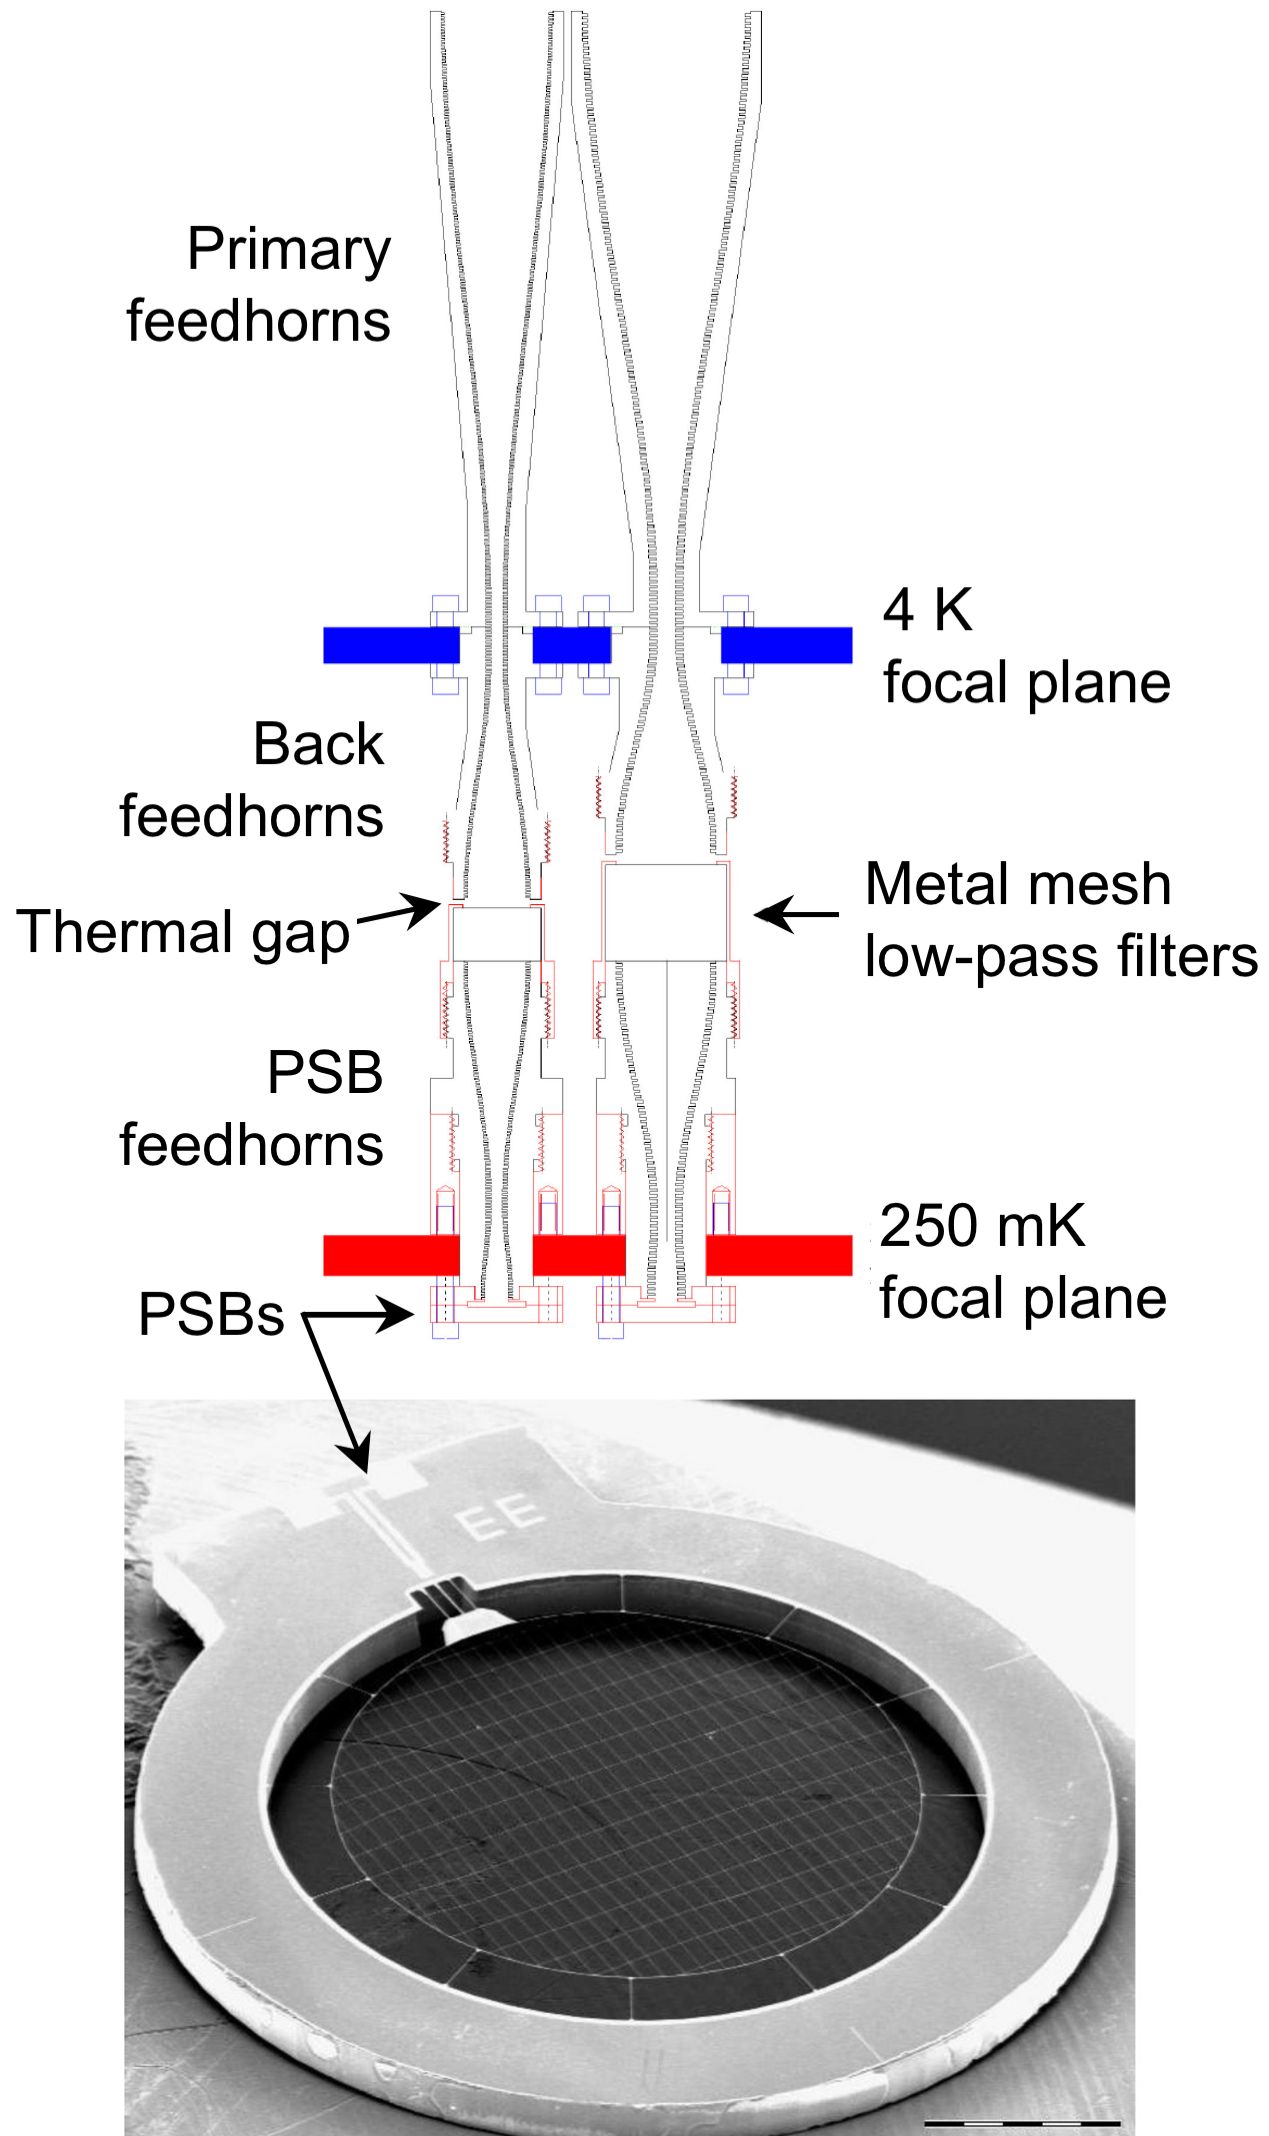
\includegraphics[width=0.35\textwidth]{figures/DirectAbsorbing.png}  %% figure was 2.5 in, .4 /textwidth is 2.6in.
%\vspace{-0.25in}
%\caption{\captiontext Top: \planck\ used horns to couple the electromagnetic radiation to its detectors. Horn coupling has been used in other experiments, and is the baseline for PICO's coupling between 555 and 799~GHz. Bottom: The photograph shows a dual-polarization, direct-absorbing bolometer from BICEP. The technology was also used with SPT-Pol and \planck-HFI for 143--343\,GHz bands.
%\label{fig:DirectAbsorbing} }
%\end{wrapfigure}

%Laboratory tests and in-flight data from balloons suggest that TES
%bolometer arrays may be more naturally robust against cosmic rays than
%the individual NTD-Ge bolometers used in \textit{Planck}. PICO will leverage lessons
%learned from \textit{Planck} and ensure robust thermal sinking of
%detector array substrates. Cosmic-ray
%glitches have fast recovery times and low coincidence rates
%\citep{SPIDER2018,Filippini_inprep}. Residual risk can be retired with 100\,mK
%testing where the array heat sinking may be weaker, and beam-line
%tests to simulate the expected flight environment.

%\subsection{Multiplexing}
%\label{sec:multiplexing}

%More than ten experiments have used time-domain multiplexer (TDM) readout. SCUBA2 on JCMT has 10,000 pixels, nearly as many detectors as planned for PICO~\citep{Holland2013}. Most of these experiments have used 32-row multiplexing. Recently ACT has expanded this to 64-row multiplexing~\citep{Henderson2016}.

%PICO's sensitivity requirements dictate the use of 13,000 transition-edge-sensor bolometers and a multiplexed system.  Our baseline design is to use TDM readout with 128 switched rows per readout column (TDM-128$\times$). The leap to TDM-128$\times$ requires: \\
%$\bullet$ development of fast-switched room temperature electronics; and \\
%$\bullet$ system engineering of room temperature to cryogenic row-select cabling to ensure sufficiently fast row-switch settling times.

%The historical row revisit rate for bolometric instruments using 32$\times$ TDM has been 25\,kHz \cite[e.g.,][]{BICEP2015}. However, X-ray instruments using TDM routinely switch between rows at 6.25~MHz~\citep{Doriese2016}. The PICO baseline assumes a 6.25~MHz switch rate and TDM-128$\times$, which dictates a row-revisit rate %(effective sampling rate) 
%of 48.8\,kHz. To limit aliased noise, PICO implements low-pass filters in each readout channel with a bandwidth of 6\,kHz, dictated by detector stability considerations and the required $\sim1$\,kHz signal bandwidth.  With these parameters and using the same TDM multiplexer SQUID design, the increased total noise due to aliasing is less than 15\,\% and is included in our detector noise budget.  The system engineering study will culminate in a demonstration of TDM-128$\times$ SQUID aliased noise below PICO detector sensitivity requirements.


%\subsection{Technology Descopes}
%\label{sec:technology_descopes} %5.3

%A descope from three-color sinuous antenna/lenslet-coupled pixels to two-color horn-coupled, or to single color antenna-array pixels remains a viable alternative should the three-color technology not mature as planned. In both alternative options, bands above 555~GHz are the same as the baseline. For the lower frequencies, the two-color horn-coupled pixel option contains 8,840 detectors and has 19 colors. Because horns have a $2.3:1$ bandwidth, each of the two bands in a pixel has 35\,\% bandwidth (compared to the baseline 25\,\%), which compensates for pixel count, resulting in 0.61\,$\mu$K$_{\rm CMB}$\,arcmin aggregate CBE map depth. This is the same as the three-color CBE map depth, and affords the same $40\,\%$ margin relative to the 0.87\,$\mu$K$_{\rm CMB}$\,arcmin baseline requirement (Table~\ref{tab:bands}). Detailed analysis would be performed to assess the impact of the coarser spectral resolution on signal component separation. Single color antenna-array pixels can have higher packing density than the other two architectures. This option has 6,540 detectors, 21 colors, each with 30\,\% bandwidth, and a noise level of 0.74\,$\mu$K$_{\rm CMB}$\,arcmin, leaving only 17\% noise margin relative to the requirement. 

%A descope from three-color sinuous antenna/lenslet-coupled pixels to two-color horn-coupled pixels remain a viable alternative should the three-color technology not mature as planned. We have a design for a PICO-size focal-plane with two-color horn-coupled pixels at the lower frequencies and the baseline one-color pixels at the higher frequencies. It contains 8,840 detectors (compared to the baseline with 12,966) and has 19 colors (baseline has 21 colors). Because horns have a $2.3:1$ bandwidth, each of the two bands in a pixel has 35\,\% bandwidth (compared to the baseline 25\,\%), which compensates for pixel count, resulting in 0.61\,$\mu$K$_{\rm CMB}$\,arcmin aggregate CBE map depth, which is the same as the three-color CBE map depth, and affords the same $40\,\%$ margin relative to the 0.87\,$\mu$K$_{\rm CMB}$\,arcmin baseline requirement (Table~\ref{tab:bands}). Detailed analysis would be performed to assess the impact of the coarser spectral resolution on signal component separation (\S\,\ref{sec:signal_separation}).

%\subsection{Enhancing Technologies}
%\label{sec:enhancing_technologies} %5.4

%The following technologies are neither required nor assumed by the PICO baseline concept. However, they represent opportunities to extend scientific capabilities or simplify engineering.

%PICO baselines TDM readout because of its relative maturity and demonstrated sensitivity and stability in relevant science missions. Lab tests of frequency-domain multiplexing (FDM) give comparable performance with higher multiplexing factors and lower thermal loads on cryogenic stages relative to TDM, but with higher ambient temperature power consumption. Suborbital experiments such as SPT-3G are using FDM to read out focal planes comparable in size to PICO.

%Microwave frequency SQUID multiplexing can increase the multiplexing density and reduce the number of wires between the 4\,K and ambient temperature stages~\citep{Dober2017,Irwin2004}. Kinetic inductance detectors and Thermal KIDs can further reduce the wire count, obviate the need for SQUID-based amplifiers, and simplify integration by integrating the multiplexing function on the same substrate as the detectors~\citep{McCarrick2018,Steinbach2018,Johnson2018}. The cost to develop these technologies is \$3--4M/year, with a high chance of reaching TRL-5 before Phase~A.
%\costfootnote

%\end{document}
